\documentclass[10pt]{article}
\usepackage[utf8]{inputenc}
\usepackage[T1]{fontenc}
\usepackage{amsmath}
\usepackage{amsfonts}
\usepackage{amssymb}
\usepackage[version=4]{mhchem}
\usepackage{stmaryrd}
\usepackage{graphicx}
\usepackage[export]{adjustbox}

\DeclareUnicodeCharacter{00D7}{\ifmmode\times\else{$\times$}\fi}

\begin{document}

\section*{Theory 13: 'LISA'}
The Laser Interferometer Space Antenna (LISA) is a proposed experiment to detect low-frequency gravitational waves. It consists of three spacecraft arranged in an equilateral triangle. A passing gravitational wave changes the distance between the spacecraft, which can be precisely measured (more details are given in the notes below).\\
One of the sources of low-frequency gravitational waves are compact binary star systems, for example binary white dwarfs. Such a system was recently discovered at a distance of 2.34 kpc from the Sun. The orbital period of the binary was found to be 414.79 s and is changing at a rate of $-7.49 \times 10^{-4} \mathrm{~s} \mathrm{yr}^{-1}$ due to the emission of gravitational waves.\\
(a) Check if this binary system can be detected by LISA.\\
(b) Calculate the chirp mass.\\
(c) Determine the masses of both components knowing that the ratio between the radius of one of the components to the semi-major axis of the orbit is 0.139 , and assuming both components follow the mass-radius relation for white dwarfs given in the table below.\\
(15 points)\\
(Total: 45 points)

\section*{Notes:}
\begin{enumerate}
  \item A binary star system with an orbital period $P$ emits gravitational waves with a frequency of $f=2 / P$.
  \item LISA measures a dimensionless quantity called the characteristic strain amplitude, $S$, given by
\end{enumerate}

$$
S=h \sqrt{f T_{\mathrm{obs}}},
$$

where $T_{\text {obs }}=4 \mathrm{yr}$ is the expected duration of the mission. $h$ is the gravitational wave strain, given by:

$$
h=\frac{2(G \mathcal{M})^{5 / 3}(\pi f)^{2 / 3}}{c^{4} D},
$$

where $\mathcal{M}$ is the so-called chirp mass, $f$ is the frequency of the gravitational wave and $D$ is the distance to the system. If we denote the masses of the components of the binary as $M_{1}$ and $M_{2}$, then the chirp mass is given by:

$$
\mathcal{M}=\frac{\left(M_{1} M_{2}\right)^{3 / 5}}{\left(M_{1}+M_{2}\right)^{1 / 5}}
$$

The expected sensitivity of LISA as a function of a gravitational wave frequency is presented on the figure below.\\
3. The semi-major axis $a$ of the binary system changes due to the emission of gravitational waves at a rate:

$$
\frac{\Delta a}{\Delta t}=-\frac{64}{5} \frac{G^{3}}{c^{5}} \frac{M_{1} M_{2}\left(M_{1}+M_{2}\right)}{a^{3}} .
$$

\begin{center}
\begin{tabular}{cc}
\hline\hline
$M\left(M_{\odot}\right)$ & $R\left(R_{\odot}\right)$ \\
\hline
0.48 & 0.0144 \\
0.50 & 0.0147 \\
0.52 & 0.0150 \\
0.54 & 0.0153 \\
0.56 & 0.0156 \\
0.58 & 0.0159 \\
0.60 & 0.0162 \\
0.62 & 0.0165 \\
0.64 & 0.0168 \\
\hline
\end{tabular}
\end{center}

Mass-radius relation for white dwarfs based on theoretical models of Althaus et al. (2013) for white dwarfs of $\log _{g}=7.7$.\\
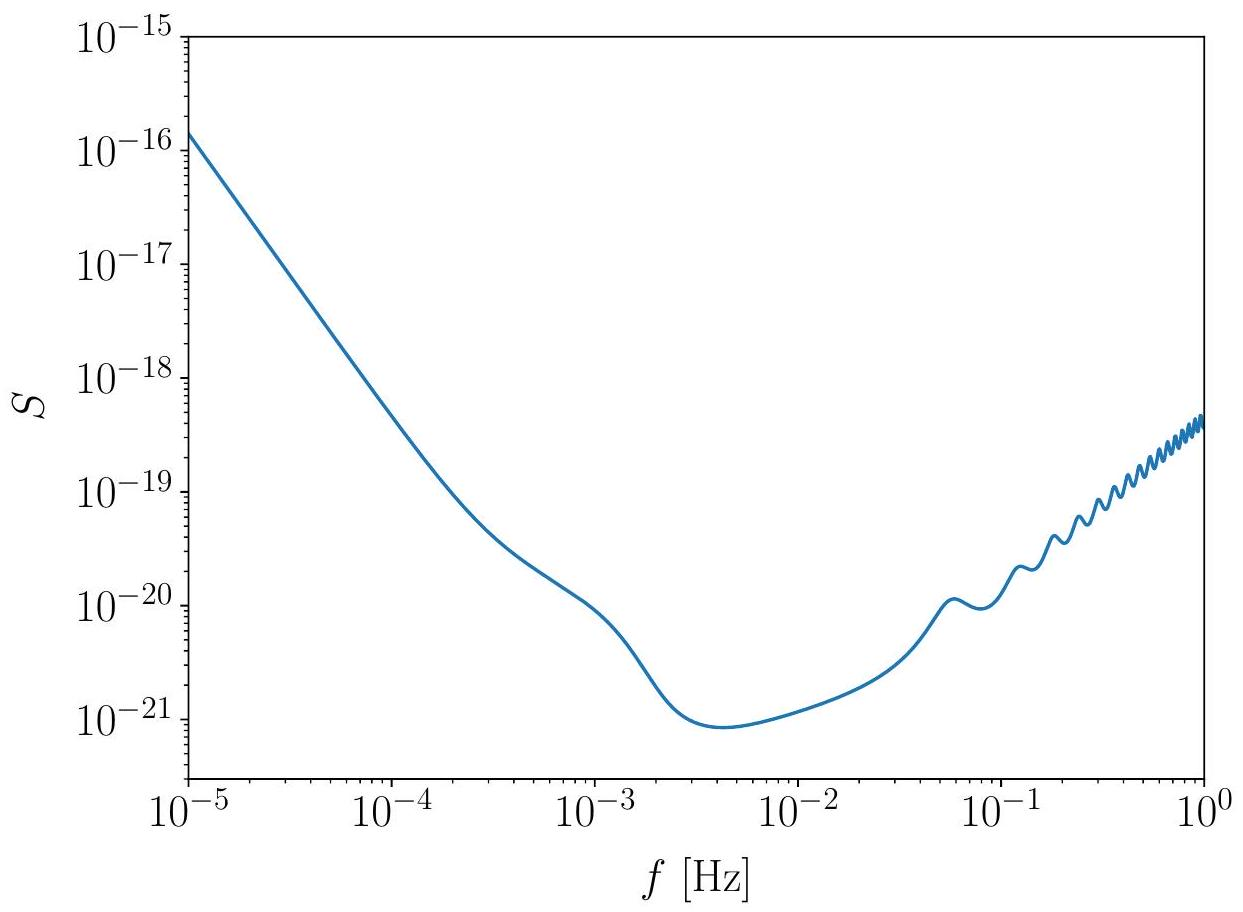
\includegraphics[max width=\textwidth, center]{2025_09_11_f1204e5353f2ce302459g-08}

The expected sensitivity of LISA as a function of gravitational wave frequency.

\end{document}